\documentclass[12pt]{article}
\usepackage[margin=0.75in]{geometry}
\usepackage{graphicx}
\usepackage{float}
\setlength{\parindent}{0mm}

\begin{document}

{\centering
\large Physics I: Lab 04 \par
\large Forces \par
}
\hfill \break \vspace{-4mm}

In this lab you will investigate several applications of Newton's second law by calculating expected outcomes and comparing to (simulated) experiments.

Some comments:
\begin{enumerate}
\item When doing calculations, you treat objects like points, so in your simulations you should make your objects relatively small to achieve better results.
\item Each object in I.P. has coefficients of friction under its properties. When two objects are in contact, I.P. calculates the friction based on the smaller of the two values.
\item A stopwatch feature is available in I.P. under Measure $\rightarrow$ Time.
\end{enumerate}

\underline{\textbf{Part 1}} \par
For each diagram below, use a ruler to accurately draw the x and y components of the given vector.
Also use a ruler and protractor to measure the magnitudes $v$, $v_x$, and $v_y$, and at least one relevant angle.
Also write down the sign (positive or negative) of each component.
Confirm your measurements using the Pythagorean Theorem and trigonometry functions.
%
\begin{figure}[H]
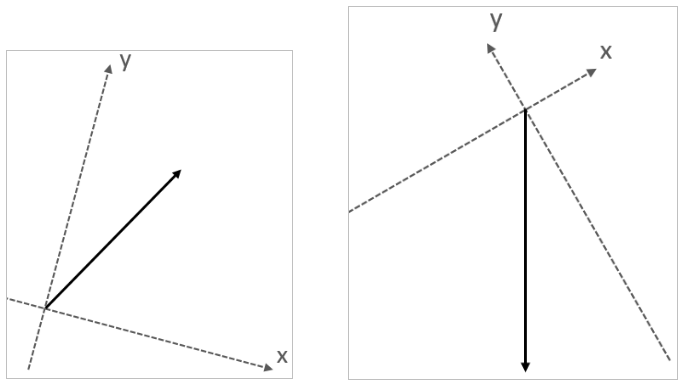
\includegraphics[scale=0.70]{figures/fig1.png}
\end{figure}

\underline{\textbf{Part 2}} \par
Create an inclined ramp experiment.
Choose reasonable values for the angle of incline and the coefficients of friction (should be non-zero but small enough that the block slides). 
%
\begin{figure}[H]
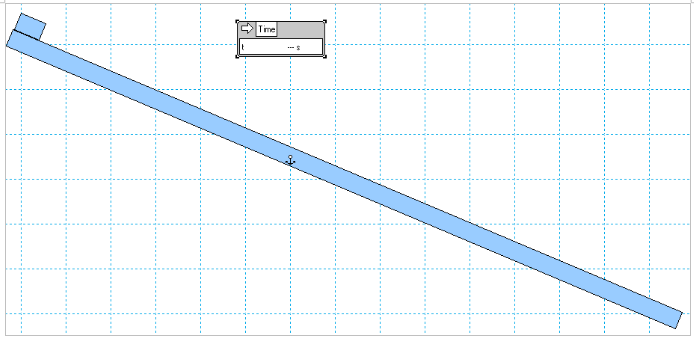
\includegraphics[scale=0.70]{figures/fig2a.png}
\end{figure}
%
Calculate how long the block should take to travel some distance along the ramp.
Run your experiment and compare results.
Make sure to turn tracking on and to record relevant information and screenshots.
%
\begin{figure}[H]
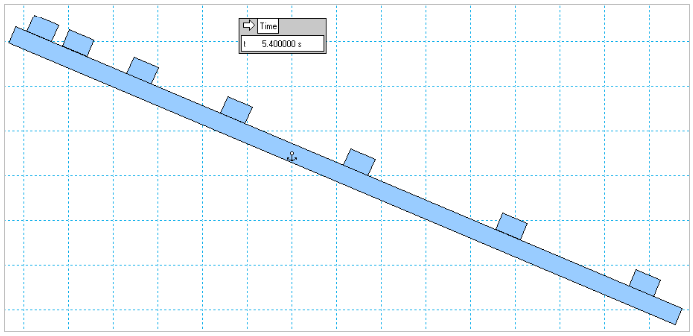
\includegraphics[scale=0.70]{figures/fig2b.png}
\end{figure}

\underline{\textbf{Part 3}} \par
Create the experiment shown below.
Let the bottom block be $m_1$ and the top block be $m_2$.
The floor is a frictionless surface, however, some friction exists between $m_1$ and $m_2$.
A constant horizontal force, $F$, is applied to $m_1$.
If the force is small, then the friction between the two blocks keeps them together; but if the force is large enough, then block 1 slides out from underneath block 2.
Play around with some settings to get a feel for this.
Next, choose some reasonable values for $m_1$, $m_2$, and $F$.
Calculate the coefficient of static friction such that the blocks are right on the brink of slipping, and set this value in the experiment.
Run the experiment several times, changing slightly a few values to confirm that you found the correct coefficient of friction.

Note: here we are not very interested in the coefficient of kinetic friction, but to avoid bugs in IP make sure it is equal to the coefficient of static friction.
%
\begin{figure}[H]
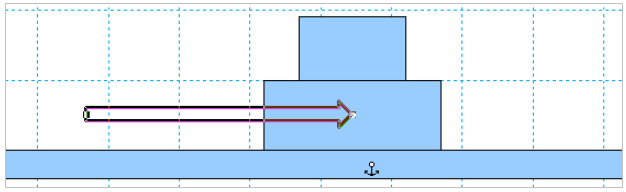
\includegraphics[scale=0.70]{figures/fig3.png}
\end{figure}

\end{document}
